\chapter{System Design}

\section{System Architecture}
\subsection{Overview}
The Nexora e-commerce platform follows a three-tier architecture:
\begin{itemize}
    \item Presentation Layer (Frontend)
    \item Application Layer (Backend)
    \item Data Layer (Database)
\end{itemize}

\begin{figure}[h]
    \centering
    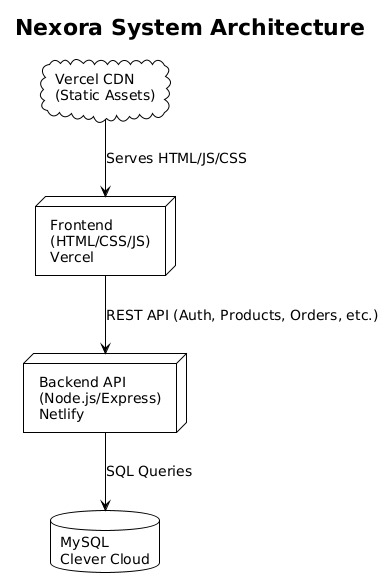
\includegraphics[width=0.8\textwidth]{SystemArchitecture.jpg}
    \caption{System Architecture Overview}
    \label{fig:system-architecture}
\end{figure}

\subsection{Component Diagram}
\begin{itemize}
    \item Frontend Components:
    \begin{itemize}
        \item User Interface
        \item Client-side Logic
        \item API Integration
    \end{itemize}
    \item Backend Components:
    \begin{itemize}
        \item API Server
        \item Business Logic
        \item Authentication Service
        \item File Service
    \end{itemize}
    \item Database Components:
    \begin{itemize}
        \item Data Storage
        \item Query Engine
        \item Backup System
    \end{itemize}
\end{itemize}

\section{Frontend Architecture}
\subsection{Component Structure}
\begin{itemize}
    \item Pages:
    \begin{itemize}
        \item Home
        \item Product Listing
        \item Product Details
        \item Cart
        \item Checkout
        \item User Dashboard
        \item Admin Panel
    \end{itemize}
    \item Components:
    \begin{itemize}
        \item Navigation
        \item Product Cards
        \item Forms
        \item Modals
        \item Notifications
    \end{itemize}
\end{itemize}

\begin{figure}[h]
    \centering
    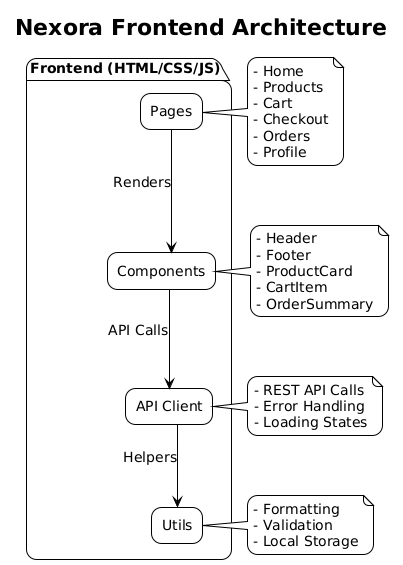
\includegraphics[width=0.8\textwidth]{FrontendArchitecture.png}
    \caption{Frontend Architecture}
    \label{fig:frontend-architecture}
\end{figure}

\section{Backend Architecture}
\subsection{API Design}
\begin{itemize}
    \item RESTful Endpoints
    \item Resource-based Routing
    \item Middleware Pipeline
    \item Error Handling
\end{itemize}

\subsection{Service Layer}
\begin{itemize}
    \item Authentication Service
    \item Product Service
    \item Order Service
    \item User Service
    \item File Service
\end{itemize}

\begin{figure}[h]
    \centering
    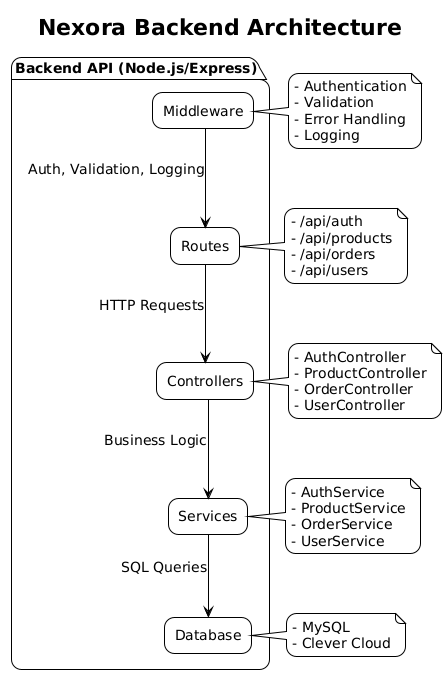
\includegraphics[width=0.8\textwidth]{BackendArchitecture.png}
    \caption{Backend Architecture}
    \label{fig:backend-architecture}
\end{figure}

\section{Database Design}
\subsection{Entity Relationship Diagram}
\begin{itemize}
    \item Core Entities:
    \begin{itemize}
        \item Users
        \item Products
        \item Orders
        \item Categories
    \end{itemize}
    \item Relationships:
    \begin{itemize}
        \item User-Order (1:N)
        \item Product-Category (M:N)
        \item Order-Product (M:N)
    \end{itemize}
\end{itemize}

\begin{figure}[h]
    \centering
    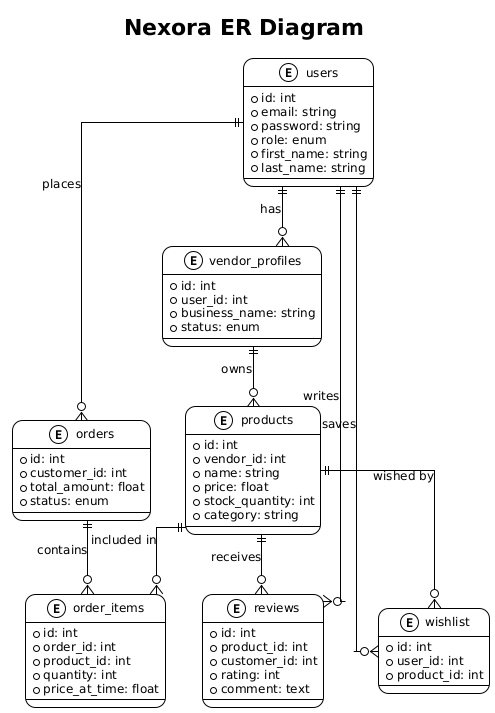
\includegraphics[width=0.8\textwidth]{ER_DiagramDetailed.png}
    \caption{Entity-Relationship Diagram}
    \label{fig:er-diagram}
\end{figure}

\section{Class Diagram}
\subsection{Core Classes}
\begin{itemize}
    \item User:
    \begin{itemize}
        \item Properties: id, name, email, role
        \item Methods: register(), login(), updateProfile()
    \end{itemize}
    \item Product:
    \begin{itemize}
        \item Properties: id, name, price, description
        \item Methods: create(), update(), delete()
    \end{itemize}
    \item Order:
    \begin{itemize}
        \item Properties: id, userId, total, status
        \item Methods: create(), updateStatus(), calculateTotal()
    \end{itemize}
\end{itemize}

\begin{figure}[h]
    \centering
    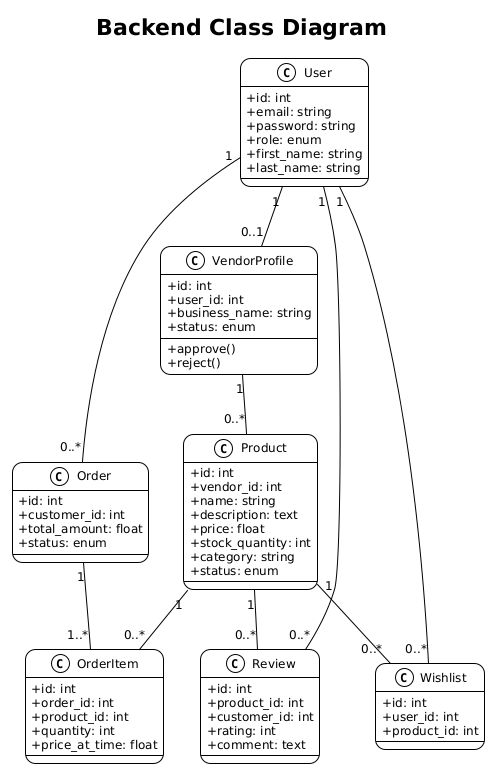
\includegraphics[width=0.8\textwidth]{DetailedClassDiagram.png}
    \caption{Detailed Class Diagram}
    \label{fig:class-diagram}
\end{figure}

\section{Sequence Diagrams}
\begin{figure}[h]
    \centering
    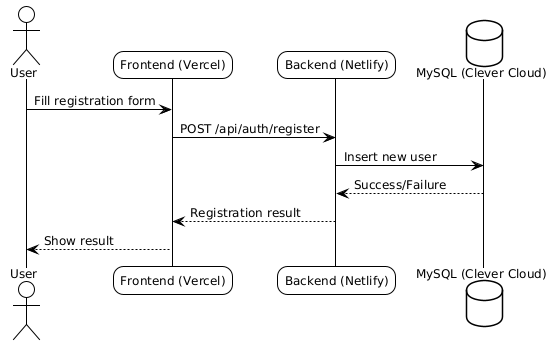
\includegraphics[width=0.7\textwidth]{Sequence_DiagramUsee_Registration.png}
    \caption{Sequence Diagram: User Registration}
    \label{fig:sd-registration}
\end{figure}

\begin{figure}[h]
    \centering
    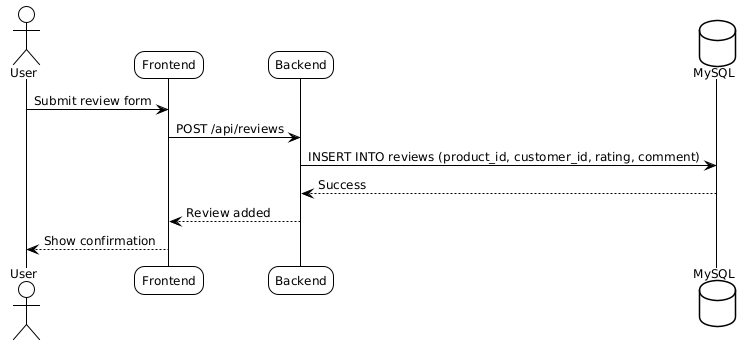
\includegraphics[width=0.7\textwidth]{SDWriteReview.png}
    \caption{Sequence Diagram: Write Review}
    \label{fig:sd-write-review}
\end{figure}

\begin{figure}[h]
    \centering
    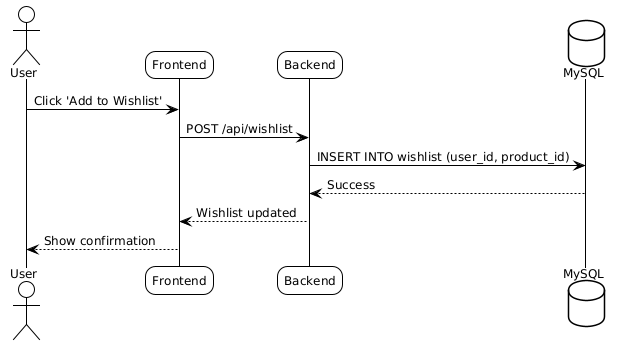
\includegraphics[width=0.7\textwidth]{SDAddtoWishlist.png}
    \caption{Sequence Diagram: Add to Wishlist}
    \label{fig:sd-add-wishlist}
\end{figure}

\begin{figure}[h]
    \centering
    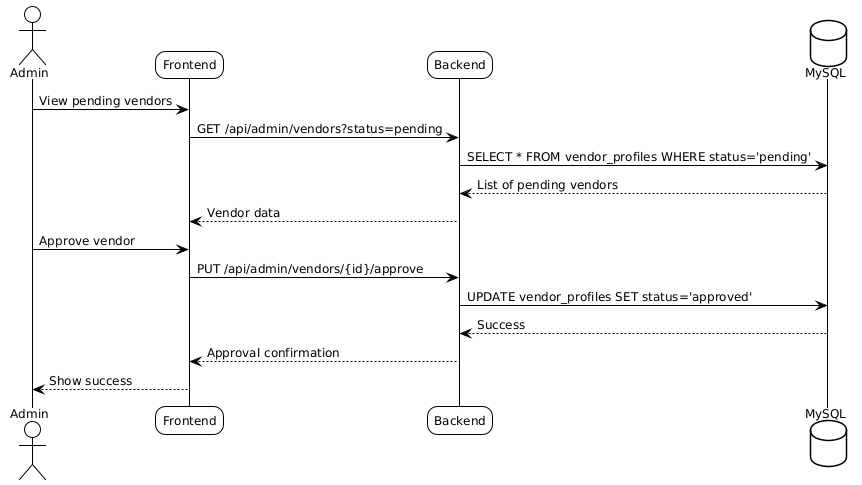
\includegraphics[width=0.7\textwidth]{SDVendor Approval.png}
    \caption{Sequence Diagram: Vendor Approval}
    \label{fig:sd-vendor-approval}
\end{figure}

\begin{figure}[h]
    \centering
    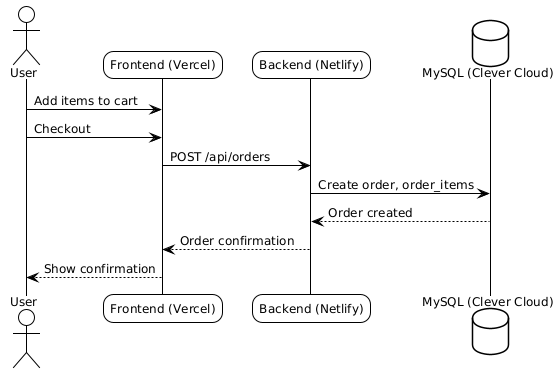
\includegraphics[width=0.7\textwidth]{Place_Order.png}
    \caption{Sequence Diagram: Place Order}
    \label{fig:sd-place-order}
\end{figure}

\section{Security Design}
\subsection{Authentication}
\begin{itemize}
    \item JWT-based authentication
    \item Password hashing
    \item Session management
    \item Role-based access control
\end{itemize}

\subsection{Data Protection}
\begin{itemize}
    \item Input validation
    \item SQL injection prevention
    \item XSS protection
    \item CSRF protection
\end{itemize}

\section{Performance Considerations}
\subsection{Optimization Strategies}
\begin{itemize}
    \item Caching:
    \begin{itemize}
        \item Browser caching
        \item API response caching
        \item Database query caching
    \end{itemize}
    \item Load Balancing:
    \begin{itemize}
        \item Horizontal scaling
        \item Request distribution
        \item Session management
    \end{itemize}
    \item Database Optimization:
    \begin{itemize}
        \item Indexing
        \item Query optimization
        \item Connection pooling
    \end{itemize}
\end{itemize}

\section{Deployment Architecture}
\subsection{Infrastructure}
\begin{itemize}
    \item Web Server
    \item Application Server
    \item Database Server
    \item File Storage
\end{itemize}

\subsection{Monitoring}
\begin{itemize}
    \item Performance monitoring
    \item Error tracking
    \item User analytics
    \item Security monitoring
\end{itemize}
